% This file was created by matlab2tikz.
%
%The latest updates can be retrieved from
%  http://www.mathworks.com/matlabcentral/fileexchange/22022-matlab2tikz-matlab2tikz
%where you can also make suggestions and rate matlab2tikz.
%
\definecolor{mycolor1}{rgb}{0.00000,0.44700,0.74100}%
\definecolor{mycolor2}{rgb}{0.85000,0.32500,0.09800}%
\definecolor{mycolor3}{rgb}{0.92900,0.69400,0.12500}%
\definecolor{mycolor4}{rgb}{0.49400,0.18400,0.55600}%
%
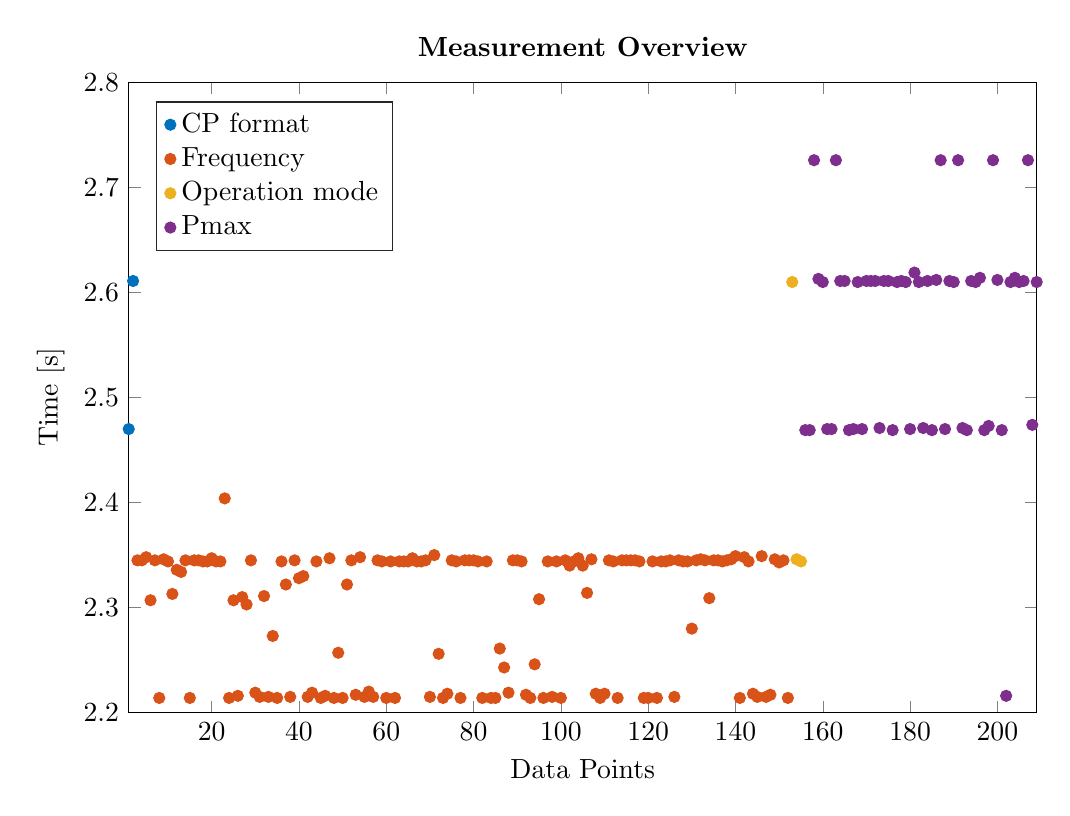
\begin{tikzpicture}

\begin{axis}[%
width=0.951\textwidth,
height=0.66\textwidth,
at={(0\textwidth,0\textwidth)},
scale only axis,
xmin=1,
xmax=209,
xlabel={Data Points},
ymin=2.2,
ymax=2.8,
ylabel={Time [s]},
axis background/.style={fill=white},
title style={font=\bfseries},
title={Measurement Overview},
legend style={at={(0.03,0.97)},anchor=north west,legend cell align=left,align=left,draw=white!15!black},
y tick label style={/pgf/number format/fixed}
]
\addplot [color=mycolor1,only marks,mark=*,mark options={solid}]
  table[row sep=crcr]{%
1	2.47\\
2	2.611\\
};
\addlegendentry{CP format};

\addplot [color=mycolor2,only marks,mark=*,mark options={solid}]
  table[row sep=crcr]{%
3	2.345\\
4	2.345\\
5	2.348\\
6	2.307\\
7	2.345\\
8	2.214\\
9	2.346\\
10	2.344\\
11	2.313\\
12	2.336\\
13	2.334\\
14	2.345\\
15	2.214\\
16	2.345\\
17	2.345\\
18	2.344\\
19	2.344\\
20	2.347\\
21	2.344\\
22	2.344\\
23	2.404\\
24	2.214\\
25	2.307\\
26	2.216\\
27	2.31\\
28	2.30299999999999\\
29	2.345\\
30	2.219\\
31	2.215\\
32	2.31099999999999\\
33	2.215\\
34	2.273\\
35	2.214\\
36	2.344\\
37	2.32199999999999\\
38	2.215\\
39	2.345\\
40	2.328\\
41	2.33\\
42	2.215\\
43	2.219\\
44	2.344\\
45	2.214\\
46	2.216\\
47	2.347\\
48	2.214\\
49	2.25699999999999\\
50	2.214\\
51	2.32199999999999\\
52	2.345\\
53	2.217\\
54	2.348\\
55	2.215\\
56	2.22\\
57	2.215\\
58	2.345\\
59	2.344\\
60	2.214\\
61	2.344\\
62	2.214\\
63	2.344\\
64	2.344\\
65	2.344\\
66	2.347\\
67	2.344\\
68	2.344\\
69	2.345\\
70	2.215\\
71	2.35\\
72	2.256\\
73	2.214\\
74	2.218\\
75	2.345\\
76	2.344\\
77	2.214\\
78	2.345\\
79	2.345\\
80	2.345\\
81	2.344\\
82	2.214\\
83	2.344\\
84	2.214\\
85	2.214\\
86	2.261\\
87	2.243\\
88	2.219\\
89	2.345\\
90	2.345\\
91	2.344\\
92	2.217\\
93	2.214\\
94	2.246\\
95	2.308\\
96	2.214\\
97	2.344\\
98	2.215\\
99	2.344\\
100	2.214\\
101	2.345\\
102	2.34\\
103	2.344\\
104	2.347\\
105	2.34\\
106	2.31399999999999\\
107	2.346\\
108	2.218\\
109	2.214\\
110	2.218\\
111	2.345\\
112	2.344\\
113	2.214\\
114	2.345\\
115	2.345\\
116	2.345\\
117	2.345\\
118	2.344\\
119	2.214\\
120	2.214\\
121	2.344\\
122	2.214\\
123	2.344\\
124	2.344\\
125	2.345\\
126	2.215\\
127	2.345\\
128	2.344\\
129	2.344\\
130	2.28\\
131	2.345\\
132	2.346\\
133	2.345\\
134	2.309\\
135	2.345\\
136	2.345\\
137	2.344\\
138	2.345\\
139	2.346\\
140	2.349\\
141	2.214\\
142	2.348\\
143	2.344\\
144	2.218\\
145	2.215\\
146	2.349\\
147	2.215\\
148	2.217\\
149	2.346\\
150	2.343\\
151	2.345\\
152	2.214\\
};
\addlegendentry{Frequency};

\addplot [color=mycolor3,only marks,mark=*,mark options={solid}]
  table[row sep=crcr]{%
153	2.61\\
154	2.346\\
155	2.344\\
};
\addlegendentry{Operation mode};

\addplot [color=mycolor4,only marks,mark=*,mark options={solid}]
  table[row sep=crcr]{%
156	2.469\\
157	2.469\\
158	2.726\\
159	2.613\\
160	2.61\\
161	2.47\\
162	2.47\\
163	2.726\\
164	2.611\\
165	2.611\\
166	2.469\\
167	2.47\\
168	2.61\\
169	2.47\\
170	2.611\\
171	2.611\\
172	2.611\\
173	2.471\\
174	2.611\\
175	2.611\\
176	2.469\\
177	2.61\\
178	2.611\\
179	2.61\\
180	2.47\\
181	2.619\\
182	2.61\\
183	2.471\\
184	2.611\\
185	2.469\\
186	2.612\\
187	2.726\\
188	2.47\\
189	2.611\\
190	2.61\\
191	2.726\\
192	2.471\\
193	2.469\\
194	2.611\\
195	2.61\\
196	2.614\\
197	2.469\\
198	2.473\\
199	2.726\\
200	2.612\\
201	2.469\\
202	2.216\\
203	2.61\\
204	2.614\\
205	2.61\\
206	2.611\\
207	2.726\\
208	2.474\\
209	2.61\\
};
\addlegendentry{Pmax};

\end{axis}
\end{tikzpicture}%